\documentclass{standalone}

\usepackage[english]{babel}
\usepackage[utf8x]{inputenc}
% Custom Font - Harding
\usepackage{fontspec}
\setmainfont{News Gothic Std}[Scale=1]

\usepackage{tikz,pgf} %and any other packages or tikzlibraries your picture needs
\usepackage{amsfonts}
\usepackage{amsmath}
\usepackage{physics}
\usepackage{amssymb}
\usepackage{mathtools}
\usetikzlibrary{shapes,arrows,patterns}

\begin{document}

%%%%%%%%%%%%%%%%%%%%%%%%%%%%%%%%%%%%%%%%%%%%%%%%%%%%%%%%%%%%%%%%%%%%%%%%%%%%%%%%
%COPY HERE
%%%%%%%%%%%%%%%%%%%%%%%%%%%%%%%%%%%%%%%%%%%%%%%%%%%%%%%%%%%%%%%%%%%%%%%%%%%%%%%%



\tikzset{every picture/.style={line width=0.75pt}} %set default line width to 0.75pt        

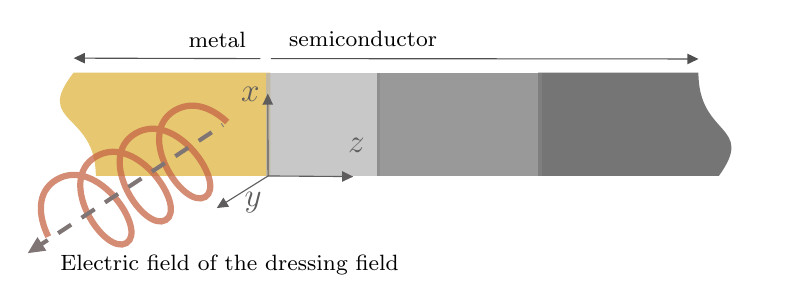
\begin{tikzpicture}[x=0.75pt,y=0.75pt,yscale=-1,xscale=1]
%uncomment if require: \path (0,403); %set diagram left start at 0, and has height of 403

%Flowchart: Document [id:dp20544451402778363] 
\draw  [draw opacity=0][fill={rgb, 255:red, 230; green, 196; blue, 104 }  ,fill opacity=0.95 ] (180.33,58.12) -- (180.33,107.87) -- (96.27,107.87) .. controls (96.27,76.77) and (65.95,82.99) .. (85.57,58.12) -- cycle ;
%Flowchart: Document [id:dp24383543064700786] 
\draw  [draw opacity=0][fill={rgb, 255:red, 91; green, 91; blue, 91 }  ,fill opacity=0.84 ] (309.33,107.87) -- (309.33,58.12) -- (386.61,58.12) .. controls (386.61,89.21) and (414.47,82.99) .. (396.44,107.87) -- cycle ;
%Shape: Rectangle [id:dp9422637204621209] 
\draw  [draw opacity=0][fill={rgb, 255:red, 181; green, 181; blue, 181 }  ,fill opacity=0.75 ] (178.27,58.12) -- (233.33,58.12) -- (233.33,107.87) -- (178.27,107.87) -- cycle ;
%Shape: Rectangle [id:dp3099632859419388] 
\draw  [draw opacity=0][fill={rgb, 255:red, 130; green, 130; blue, 130 }  ,fill opacity=0.82 ] (231.6,58.12) -- (311.33,58.12) -- (311.33,107.87) -- (231.6,107.87) -- cycle ;
%Straight Lines [id:da6577138908650908] 
\draw [color={rgb, 255:red, 80; green, 80; blue, 80 }  ,draw opacity=1 ]   (180.58,51.33) -- (383.64,51.5) ;
\draw [shift={(386.64,51.5)}, rotate = 180.05] [fill={rgb, 255:red, 80; green, 80; blue, 80 }  ,fill opacity=1 ][line width=0.08]  [draw opacity=0] (5.36,-2.57) -- (0,0) -- (5.36,2.57) -- cycle    ;
%Straight Lines [id:da6533946524084127] 
\draw [color={rgb, 255:red, 80; green, 80; blue, 80 }  ,draw opacity=1 ]   (175.58,51.33) -- (88.64,51.11) ;
\draw [shift={(85.64,51.1)}, rotate = 0.15] [fill={rgb, 255:red, 80; green, 80; blue, 80 }  ,fill opacity=1 ][line width=0.08]  [draw opacity=0] (5.36,-2.57) -- (0,0) -- (5.36,2.57) -- cycle    ;

%Straight Lines [id:da8900942762706974] 
\draw [color={rgb, 255:red, 94; green, 92; blue, 92 }  ,draw opacity=1 ]   (179.27,107.87) -- (217.29,108.15) ;
\draw [shift={(220.29,108.17)}, rotate = 180.43] [fill={rgb, 255:red, 94; green, 92; blue, 92 }  ,fill opacity=1 ][line width=0.08]  [draw opacity=0] (5.36,-2.57) -- (0,0) -- (5.36,2.57) -- cycle    ;
%Straight Lines [id:da7579554888233628] 
\draw [color={rgb, 255:red, 94; green, 92; blue, 92 }  ,draw opacity=1 ]   (179.27,107.87) -- (179.14,71.19) ;
\draw [shift={(179.13,68.19)}, rotate = 89.8] [fill={rgb, 255:red, 94; green, 92; blue, 92 }  ,fill opacity=1 ][line width=0.08]  [draw opacity=0] (5.36,-2.57) -- (0,0) -- (5.36,2.57) -- cycle    ;
%Straight Lines [id:da8806903067171721] 
\draw [color={rgb, 255:red, 94; green, 92; blue, 92 }  ,draw opacity=1 ]   (179.27,107.87) -- (157.1,121.74) ;
\draw [shift={(154.56,123.33)}, rotate = 327.96] [fill={rgb, 255:red, 94; green, 92; blue, 92 }  ,fill opacity=1 ][line width=0.08]  [draw opacity=0] (5.36,-2.57) -- (0,0) -- (5.36,2.57) -- cycle    ;
%Shape: Spring [id:dp8013325847451054] 
\draw  [color={rgb, 255:red, 198; green, 101; blue, 70 }  ,draw opacity=0.75 ][line width=2.25]  (73.37,137.11) .. controls (68.54,127.37) and (67.49,115.43) .. (77.41,109.62) .. controls (97.26,98) and (121.33,134.16) .. (110.97,140.23) .. controls (100.61,146.29) and (76.55,110.12) .. (96.4,98.51) .. controls (116.25,86.89) and (140.31,123.05) .. (129.96,129.11) .. controls (119.6,135.17) and (95.54,99.01) .. (115.39,87.39) .. controls (135.24,75.78) and (159.3,111.94) .. (148.94,118) .. controls (138.59,124.06) and (114.52,87.9) .. (134.37,76.28) .. controls (143.04,71.21) and (152.51,75.24) .. (159.57,81.91) ;
%Straight Lines [id:da49769012034859994] 
\draw [color={rgb, 255:red, 127; green, 117; blue, 117 }  ,draw opacity=1 ][line width=1.5]  [dash pattern={on 5.63pt off 4.5pt}]  (66.84,142.86) -- (157.5,83.3) ;
\draw [shift={(63.5,145.05)}, rotate = 326.7] [fill={rgb, 255:red, 127; green, 117; blue, 117 }  ,fill opacity=1 ][line width=0.08]  [draw opacity=0] (8.13,-3.9) -- (0,0) -- (8.13,3.9) -- cycle    ;

% Text Node
\draw (139.68,37.19) node [anchor=north west][inner sep=0.75pt]  [font=\footnotesize] [align=left] {metal};
% Text Node
\draw (188.18,36.69) node [anchor=north west][inner sep=0.75pt]  [font=\footnotesize] [align=left] {semiconductor};
% Text Node
\draw (77.9,144.92) node [anchor=north west][inner sep=0.75pt]  [font=\footnotesize] [align=left] {Electric field of the dressing field};
% Text Node
\draw (216.6,88.23) node [anchor=north west][inner sep=0.75pt]  [font=\large,color={rgb, 255:red, 94; green, 92; blue, 92 }  ,opacity=1 ]  {$z$};
% Text Node
\draw (165.02,63.7) node [anchor=north west][inner sep=0.75pt]  [font=\large,color={rgb, 255:red, 94; green, 92; blue, 92 }  ,opacity=1 ]  {$x$};
% Text Node
\draw (166.65,114.3) node [anchor=north west][inner sep=0.75pt]  [font=\large,color={rgb, 255:red, 94; green, 92; blue, 92 }  ,opacity=1 ]  {$y$};


\end{tikzpicture}



%%%%%%%%%%%%%%%%%%%%%%%%%%%%%%%%%%%%%%%%%%%%%%%%%%%%%%%%%%%%%%%%%%%%%%%%%%%%%%%%
%COPY HERE
%%%%%%%%%%%%%%%%%%%%%%%%%%%%%%%%%%%%%%%%%%%%%%%%%%%%%%%%%%%%%%%%%%%%%%%%%%%%%%%%

\end{document}
